\chapter*{Example 4: Root exudation in the soil-root system}

\section*{The model}
This example investigates the transportation (convection - diffusion) of root exudation in soil and
root exudation decomposition. Initially, citrate and mucilage are considered in the modelling.

\subsection*{The soil sub-problem}

The transport of root exudation in soil is described by two equations: the Richards
equation and the transport (convection - diffussion) equations in
3D soil domain. The Richards equation is formulated in multi-phase
flow context as

\[
\frac{\partial}{\partial t}\left(\rho_{w}\Phi S\right)-\nabla\cdot\left[\rho_{w}\frac{\kappa}{\mu}K\left(\nabla p_{w}-\rho_{w}\boldsymbol{g}\right)\right]=q_{w}
\]

with $t$ - time $[s]$, $\theta$ water content, $S$ saturation,
$\Phi$ porosity, $S\phi=\theta$, $\rho_{w}$ water density, $K$
intrinsic permeability, $\mu$ dynamic viscosity, $\kappa$ relative
permeability, $q_{w}$ sink term for water uptake, $\boldsymbol{g}$
gravitational acceleration, $p_{w}$ absolute pressure of wetting
phase (water)\footnote{$p_{w}$is the absolute pressure. The matric pressure $p_{m}$ is
defined as $p_{m}=p_{w}-p_{a}$, where $p_{a}$ is the air pressure,
assumed to be constant and equal to $1x10^{5}$ Pa in this Richards
equation model. In order to have head units, we need to convert the
water potential from energy per unit volume of water (pressure) to
energy per unit weight, i.e., $h_{m}=\frac{p_{m}}{\rho_{w}\boldsymbol{g}}$}. $\theta$ and $h_{m}$ are related by the water retention curve:
$\theta:=\theta(h)$ (e.g. van Genuchten model) and $K_{c}=\frac{Kk_{r}w\varrho_{w}g}{\mu_{w}}$
. The simulation domain is a rectangular block of soil, $\Omega_{s}$,
and we prescribe uniform initial conditions and no-flux boundary conditions
at the outer faces $\partial\Omega_{s}$, i.e.,
\begin{eqnarray}
p_{w}=p_{w,0} & \text{ at } & t=0\\
\rho_{w}\frac{\kappa}{\mu}K\left(\nabla p_{w}-\rho_{w}\boldsymbol{g}\right) \cdot \mathbf{n}=0 & \text{ at } & \partial\Omega_{s}
\end{eqnarray}

The transport equation for root exudation is

\[
\phi\frac{\partial\rho_{w}X_{c}S}{\partial t}-\nabla \cdot (D\rho_{w}\nabla X_{c})-\nabla \cdot (\rho_{w}X_{c}\kappa_{r}\frac{\kappa}{\mu}(\nabla p_{w}-\rho_{w}g))=q_{c}
\]

with $X_{c}$ is mass or mole fraction of transported component (in
this example is the mass fraction of root exudation); $D$ is dispersion - diffusion
coefficient of component in soil solution and $q_{c}$ is sink term
for plant-root uptake. The inital conditions and boundary condition
as contant mass fraction at the outer soil domain:
\begin{eqnarray}
\left( -D\rho_{w}\nabla X_{c} - \rho_{w}X_{c}\kappa_{r}\frac{\kappa}{\mu}(\nabla p_{w}-\rho_{w}\mathbf{g})  \right) \cdot \mathbf{n}=0 & \text{ at the geometry boundary},
\end{eqnarray}


\subsection*{The root system sub-problem}

We solve a modified version of the Richards equation on the 1D network in 3D space that describes the root architecture. We assume that the root is fully saturated with water, i.e., S=1. We further follow the cohesion-tension theory wherein pressure gradients are the driving force for water movement from soil through plants to the atmosphere. Thus, there is negative absolute pressure inside the xylem\footnote{Water can be liquid at negative pressure (metastable) (Caupin et al. 2013). Constitutive relations e.g. between pressure and density are less known in this state (Davitt et al. 2010). However, in our simulations, we assume constant pressure}.

\begin{eqnarray}
\frac{\partial}{\partial t}\left(\rho_{w}\Phi\overbrace{S}^{=1}\right)-\nabla\cdot\left[\rho_{w}K_{x}\left(\nabla p_{w}-\rho\boldsymbol{g}\right)\right]=\rho_{w}q_{w,r},
\end{eqnarray}
with $K_{x}$ axial conductance and $q_{w,r}$ the sink term for water
uptake by an individual root segment.

We prescribe zero initial conditions and no-flux boundary conditions
at the root tips. At the root collar, we prescribe the water flux
equal to the potential transpiration rate T$_{pot}$ as long as the
pressure at the root collar is above a certain threshold value. When
the pressure at the root collar reaches this threshold value, the
boundary condition is switched to a dirichlet condition where the
pressure is prescribed to be equal to the threshold value.
\begin{eqnarray}
p_{w}=0 & \text{ at } & t=0\\
\rho_{w}K_{x}\left(\nabla p_{w}-\rho\boldsymbol{g}\right) \cdot \mathbf{n}=0 & \text{ at the root tips}\\
\rho_{w}K_{x}\left(\nabla p_{w}-\rho\boldsymbol{g}\right) \cdot \mathbf{n}=T_{pot} & \text{ at the root collar} & \text{ if }p_{w}>p_{w,c}\\
p_{w}=p_{w,c} & \text{ at the root collar} & \text{ if }p_{w}\le p_{w,c},
\end{eqnarray}
where $T_{pot}$ is the potential transpiration rate, and $p_{w,c}$
is the critical water pressure (as absolute pressure, permanent wilting
point PLUS air pressure!).

The transport of root exudation in the root system is described
by the convective diffusive equation.

\[
\phi\frac{\partial\rho X_{c}S}{\partial t}-\nabla \cdot (D\rho\nabla X_{c})-\nabla \cdot (\rho X_{c}K_{x}\nabla p_{w}-\rho\boldsymbol{g})-q_{c}=0
\]

For the boundary conditions, we describe zero flux at the root tips and free outflow boundary at the root collar.

\begin{eqnarray}
X_{c}=0 & \text{ at } & t=0\\
(-D\rho_w \nabla X_{c}-\rho_w X_{c}\left(K_{x}\nabla_w p_{w}-\rho_w\boldsymbol{g}\right)\cdot \mathbf{n}= 0 & \text{ at the root tips}\\
(-D\rho_w \nabla X_{c})\cdot \mathbf{n} = 0 & \text{ at the root collar}
\end{eqnarray}


\subsection*{Coupling the soil and the root system subproblems}

In this example, water uptake depends on both the pressures inside the soil and inside the root system. The exudates, however, are exuded into the soil; there is no uptake of exudates by the roots. Thus, the interaction is only in one direction, i.e., the sink term of exudates in the root system is equal to zero.

For each root segment, the radial flux of water $q_{w,r}$ is given by 
\begin{eqnarray}
q_{w,r}=\frac{2\pi rl}{V_r}K_{r}(p_{w,root}-p_{w,soil}),
\end{eqnarray}
where $V_r$ is the volume of the root segment, $K_{r}$ is the root hydraulic conductivity, $r$ is the root
radius, $l$ is the length of the root segment, $p_{w,root}$ is the absolute pressure inside the root segment, and $p_{w,soil}$ is the local absolute water pressure of the soil at this root segment.

Water uptake from soil is computed by summing over the root segments that lie inside each soil control volume $V_s$, i.e.,
\begin{eqnarray}
q_{w,V_s}=\sum_{i=1}^{N}\left(\frac{1}{V_s}2\pi r_{i}fl_{i}K_{r,i}(p_{w,root,i}-p_{w,soil})\right),
\end{eqnarray}
where $N$ is the number of root segments that lie inside $V_s$, $f$ is the fraction of root segment length that lies inside $V_s$.

Exudation by a growing root system is defined via the age of the root segment, only the youngest parts of the root system (i.e.the parts near the root tip) can contribute to exudation. 
Root exudation into a each soil control volume $V$ is given by summing over the exudation of each root segment that lies insice $V_s$, 

\[
q_{c,V}=\sum_{i=1}^{N}\left(\frac{1}{V_s}2\pi r_{i}f F_{ex} e^{-\text{rootAge } \tau} \right)
\])

where $N$ is the number of root segments that lie inside $V_s$, $f$ is the fraction of root segment length that lies inside $V_s$, $F_{ex}$ is the maximal exudation rate, rootAge is the age of the root segment, $\tau$ is the rate of decrease of exudation with age.

\section*{The DuMu$^{x}$ code}

In this chapter, we explain where the different terms of the model
equations can be found in the DuMu$^{x}$ code, i.e., the storage,
flux and sink terms.

\subsection*{The soil sub-problem}

The storage and flux terms are defined in the file

\begin{lstlisting}
dumux-rosi/dumux/porousmediumflow/richards2cbuffer/richards2clocalresidual.hh
\end{lstlisting}
\lstinputlisting[firstline=90,lastline=125, language=C++, caption=storage terms]{dumux-rosi/dumux/porousmediumflow/richards2cbuffer/richards2cbufferlocalresidual.hh}

The advective flux is calculated in the same file as:
\lstinputlisting[firstline=162,lastline=198, language=C++, caption=advective flux terms]{dumux-rosi/dumux/porousmediumflow/richards2cbuffer/richards2cbufferlocalresidual.hh}

The diffusive flux is calculated in the same file as:
\lstinputlisting[firstline=211,lastline=231, language=C++, caption=diffusive flux terms]{dumux-rosi/dumux/porousmediumflow/richards2cbuffer/richards2cbufferlocalresidual.hh}


the dispersionTensor is calculated in

\begin{lstlisting}
dumux-rosi/dumux/porousmediumflow/richards2cbuffer/richards2cbufferfluxvariables.hh
\end{lstlisting}
\lstinputlisting[firstline=532,lastline=570, language=C++, caption=dispersion tensor]{dumux-rosi/dumux/porousmediumflow/richards2cbuffer/richards2cbufferfluxvariables.hh}

\subsection*{The root sub-problem}

The description of the source and flux terms can be found in

\begin{lstlisting}
dumux-rosi/dumux/porousmediumflow/rootmodel1p2c/localresidual1p2c.hh
\end{lstlisting}
The storage term:
\lstinputlisting[firstline=100,lastline=125, language=C++, caption=storage term]{dumux-rosi/dumux/porousmediumflow/rootmodel1p2c/localresidual1p2c.hh}

The advective terms are computed in the same file:
\lstinputlisting[firstline=158,lastline=125, language=C++, caption=advective flux term]{dumux-rosi/dumux/porousmediumflow/rootmodel1p2c/localresidual1p2c.hh}

diffusive terms:
\lstinputlisting[firstline=203,lastline=220, language=C++, caption=advective flux term]{dumux-rosi/dumux/porousmediumflow/rootmodel1p2c/localresidual1p2c.hh}

\subsection*{Fluidsystem}

To model the transport process, it requires to set up a fluid system
with 2 components: the main component of the fluid - water and the
transport component - a solute (in this case citrate). All the chemo - physical properties of the component citrate are set in the file

\begin{lstlisting}
/dumux-rosi/dumux/material/components/anions/citrate.hh
\end{lstlisting}

in which the molar mass and diffusive coefficient can be found

\lstinputlisting[firstline=43,lastline=44, language=C++, caption={}]{dumux-rosi/dumux/material/components/anions/citrate.hh}

\lstinputlisting[firstline=43,lastline=44, language=C++, caption={}]{dumux-rosi/dumux/material/components/anions/citrate.hh}

\lstinputlisting[firstline=46,lastline=51, language=C++, caption={}]{dumux-rosi/dumux/material/components/anions/citrate.hh}

\todo[inline]{Replace with diffusion coefficient of citrate}

The fluidsystem of water and citrate is set in file

\begin{lstlisting}
/dumux-rosi/dumux/material/fluidsystems/h2ocitrate.hh
\end{lstlisting}

and must be included in both soil problem and root problem

\begin{lstlisting}
/dumux-rosi/rosi_examples/RosiRichards2cExud/soilRichards2ctestproblem.hh
/dumux-rosi/rosi_examples/RosiRichards2cExud/rootsystem1p2ctestproblem.hh
\end{lstlisting}

The sink terms are computed in the above mentioned files.
\lstinputlisting[firstline=303,lastline=337, language=C++, caption=sink term in soil subproblem]{dumux-rosi/rosi_examples/RosiRichards2cExud/soilRichards2ctestproblem.hh}

\lstinputlisting[firstline=320,lastline=379, language=C++, caption=sink term in root subproblem]{dumux-rosi/rosi_examples/RosiRichards2cExud/rootsystem1p2ctestproblem.hh}


\subsection*{The input files}

In this subsection, we summarize the required model parameters. All
parameter units are based on on absolute pressure and DuMu$^{x}$
standard units (SI).

%\begin{table}[h!]
%\caption{Model input parameters}
%\label{tab:inputs} %
%\begin{tabular}{l|c||r}
%\textbf{Parameter}  & \textbf{Units}  & \textbf{File number}\tabularnewline
%\hline
%Water density  & kg m$^{-3}$  & 1\tabularnewline
%Dynamic viscosity  & kg s$^{-1}$ m$^{-1}$ & 1\tabularnewline
%Molar mass of BaP & kg mol$^{-1}$ & 2\tabularnewline
%Diffusive coefficient of BaP & m$^{2}$s$^{-1}$ & 2\tabularnewline
%Soil porosity  & m$^{3}$ m$^{-3}$  & 4\tabularnewline
%Intrinsic soil permeability  & m$^{2}$  & 4\tabularnewline
%Residual saturation  & -  & 4\tabularnewline
%Van Genuchten $\alpha$  & Pa  & 4\tabularnewline
%Van Genuchten $n$  & -  & 4\tabularnewline
%Dispersion coefficient & m$^{2}$s$^{-1}$ & 4\tabularnewline
%Root porosity  & m$^{3}$ m$^{-3}$  & 3\tabularnewline
%Root axial conductance  & m$^{5}$ s kg$^{-1}$  & 4\tabularnewline
%Root radial conductivity  & m$^{2}$ s kg$^{-1}$  & 4\tabularnewline
%\end{tabular}
%\end{table}

\begin{enumerate}
\item \verb+dumux/dumux/material/components/simpleh2o.hh+
\item \verb+dumux-rosi/dumux/material/components/anions/citrate.hh+
\item \verb+dumux-rosi/rosi_examples/RosiRichards2cExud/rootsystemtestspatialparams.hh+
\item \verb+dumux-rosi/rosi_examples/RosiRichards2cExud/test_rosiRichards2cExud.input+
\end{enumerate}
Here is the listing of the .input-file:
\lstinputlisting[firstline=7,lastline=69, language={}, caption=input file]{dumux-rosi/rosi_examples/RosiRichards2cExud/test_rosiRichards2cExud.input}


\subsection*{Simulation}

Boundary conditions in soil domain are defined in the file
\begin{lstlisting}
    dumux-rosi/rosi_examples/RosiRichards2cExud/soilRichards2ctestproblem.hh}
\end{lstlisting}

\lstinputlisting[firstline=351,lastline=366, language=C++, caption=boundary conditions]{dumux-rosi/rosi_examples/RosiRichards2cExud/soilRichards2ctestproblem.hh}

Initial condition is homogenous field of water saturation and mass fraction of exudate
\lstinputlisting[firstline=426,lastline=435, language=C++, caption=initial conditions]{dumux-rosi/rosi_examples/RosiRichards2cExud/soilRichards2ctestproblem.hh}


The boundary conditions in root problem are set with zero flux at root tips and free out flow at root colar for tranport equation. The switch boundary condition from Neuman to Dirichlet is implemented in case xylem pressure lower than critical value.

The boundary conditions of the root problem are set with zero flux at root tips and free out flow at root colar for tranport equation. The switch boundary condition from Neuman to Dirichlet is implemented in case xylem pressure lower than critical value. This is implemented as the default boundary condition for all root problems in the file 
\begin{lstlisting}
dumux-rosi/dumux/porousmediumflow/rootmodel1p2c/problem1p2c.hh
\end{lstlisting}

\lstinputlisting[firstline=173,lastline=215, language=C++, caption=boundary conditions]{dumux-rosi/dumux/porousmediumflow/rootmodel1p2c/problem1p2c.hh}

Results: mass fraction of exudate

\noindent\begin{minipage}[c]{1\columnwidth}%
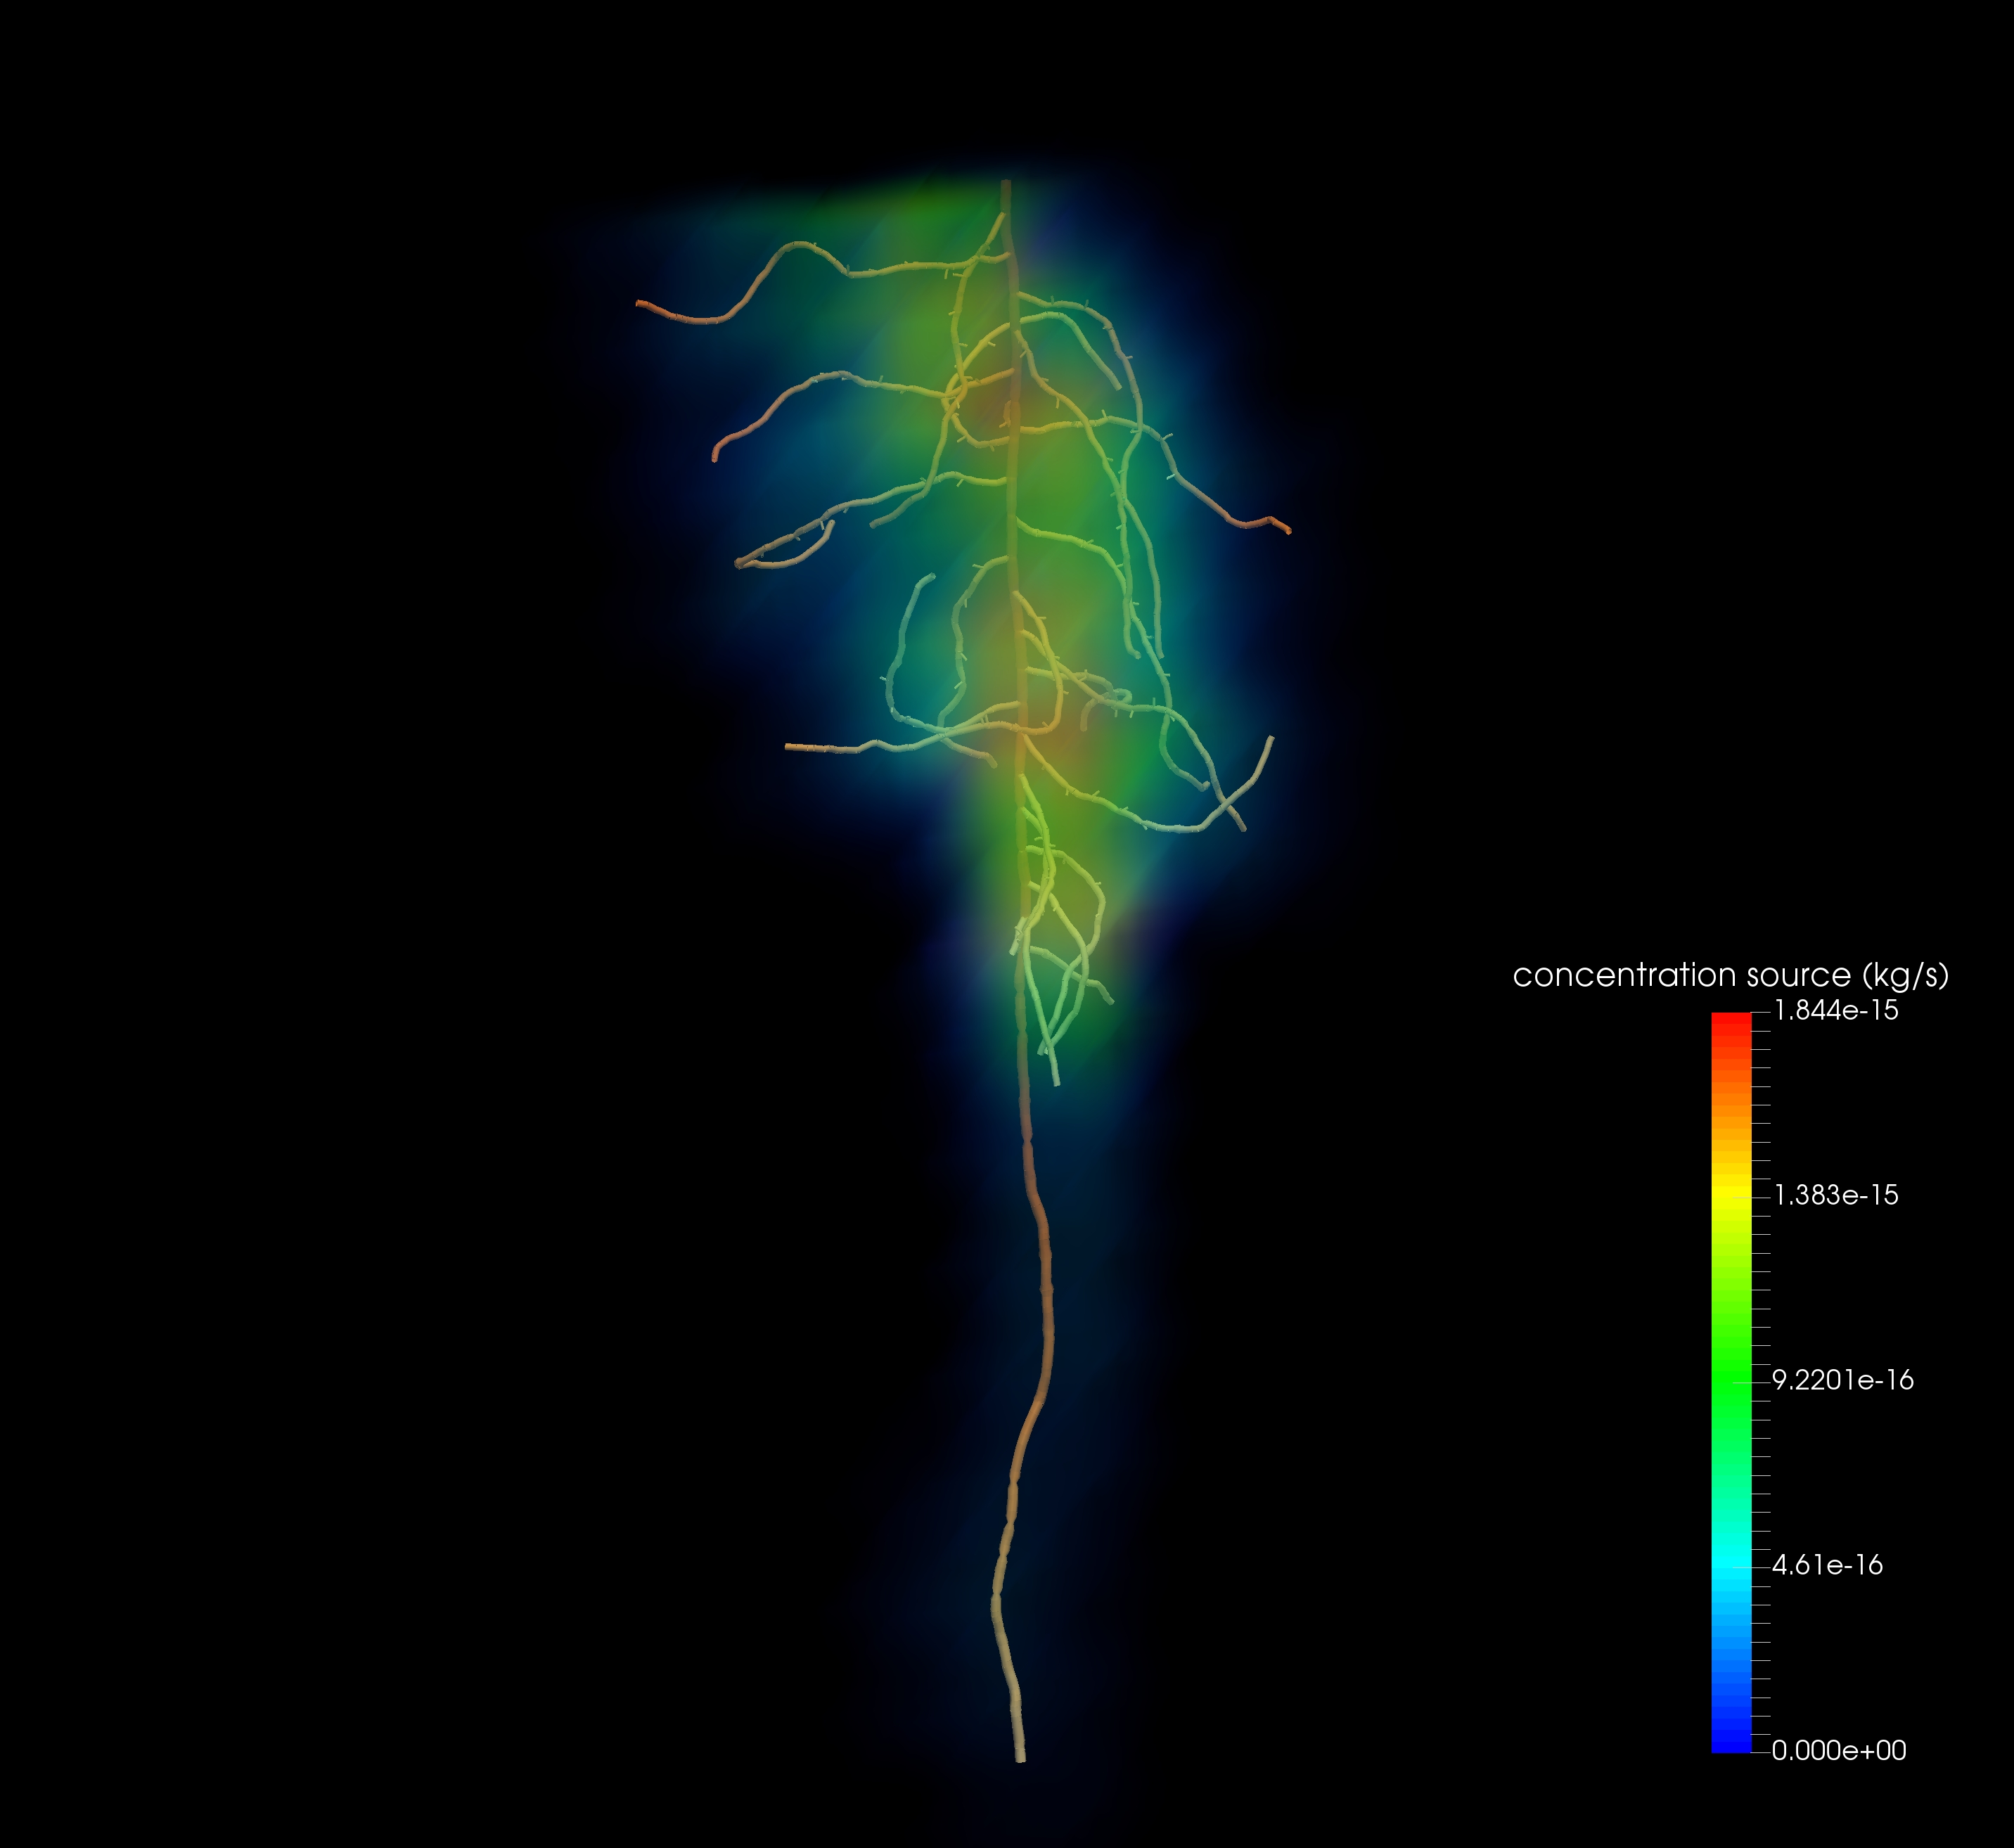
\includegraphics[width=0.9\textwidth]{example_exudates.jpg}%
\end{minipage}

\subsection*{Technical issues}

\subsubsection*{Solver}

The default solver of all dumux-rosi examples is an iterative solver.
In rosiRichards2ctestproblem the solver can be set in line 69:
\begin{lstlisting}
SET_TYPE_PROP(RosiRichardsTwoCBufferTestProblem, LinearSolver, ILU0BiCGSTABBackend<TypeTag>);
\end{lstlisting}

At moment, the properties of component tranport is setup and hard
coded. It would be better that the definition of component and all
its properties (molar density, diffusion coefficient..) be moved to
the input file for the ease of use.

